\section{Solution}
\subsection{Solution Overview}
\begin{frame}
Resilient Distributed Datasets (RDDs)
\begin{itemize}
  \item Restricted form of distributed shared memory
  \item Immutable
  \item Only built through reading stable storage or coarse-grained
  deterministic \textbf{transformations} (\texttt{map}, \texttt{filter}, \texttt{join}, \ldots)
  \item \textbf{Actions} (\texttt{count}, \texttt{collect}, \texttt{reduce},
  \ldots) either return value or write to storage
\end{itemize}
\end{frame}

\subsection{Example}
\begin{frame}
\begin{figure}
\centering
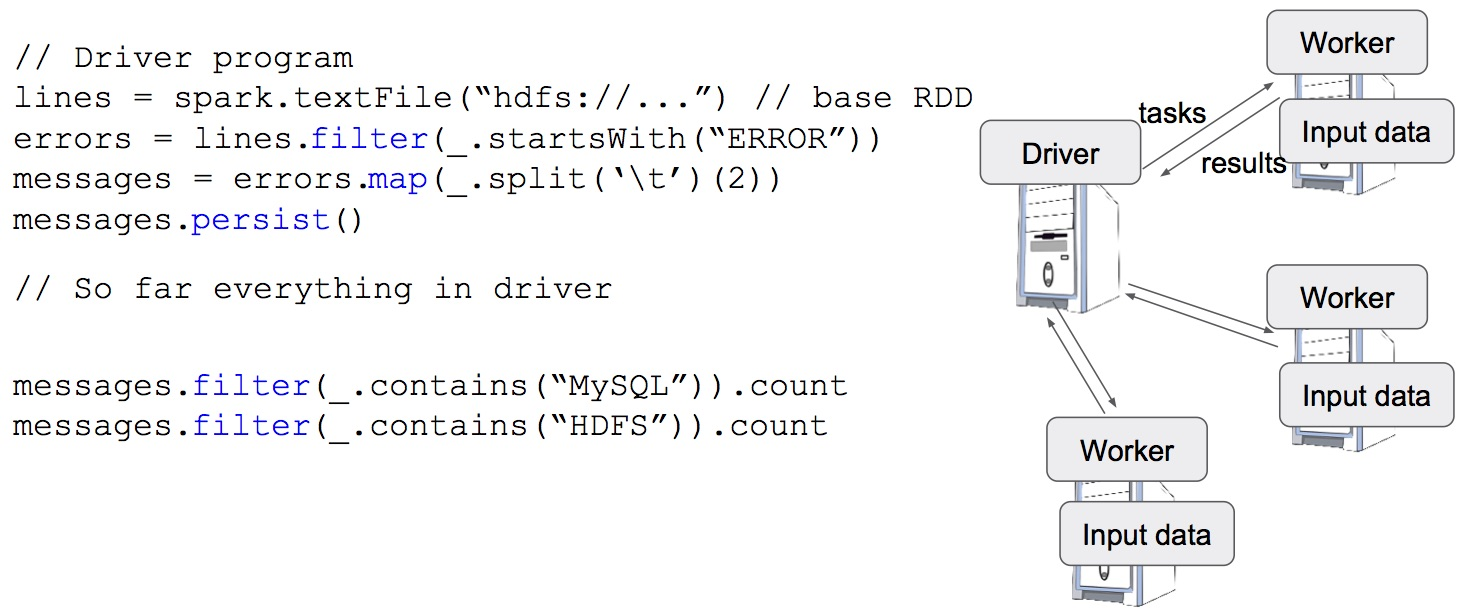
\includegraphics[width=0.9\linewidth]{figures/example1.jpg}
\caption{Load error messages from a log into memory and then interactively
search for various patterns.}
\end{figure}
\end{frame}

\begin{frame}
\begin{itemize}
  \item Transformations are lazy
  		\begin{itemize}
  		  \item Do not compute result until action is invoked
  		  \item Useful
  		\end{itemize}
\end{itemize}
\end{frame}

\begin{frame}
\begin{itemize}
  \item Users can control two other aspects,
	  \begin{itemize}
		  \item \textbf{Persistence}: keep an RDD in memory using \texttt{persist} or
		  \texttt{cache}. Can spill the RDDs to disk if not enough RAM,
		  \item \textbf{Partitioning}: an RDDs elements be partitioned across machines
		  based on a key in each record.
	  \end{itemize}
  \item In comparison with MapReduce,
  		\begin{itemize}
  		  \item map: a transformation that passes each dataset element through a
  		  function and returns a new RDD representing the results,
  		  \item reduce: an action that aggregates all the elements of the RDD using
  		  some function and returns the final result to the driver program
  		\end{itemize}
\end{itemize}
\end{frame}

% \begin{lstlisting}[language=scala]
% 	lines = spark.textFile("hdfs://...") // Base RDD
% 	errors = lines.filter(_.startsWith("ERROR")) // Transformed RDD
% 	messages = errors.map(_.split('\t')(2))
% 	messages.persist()
% 	
% 	// so far everything in the driver (master),
% 	
% 	messages.filter(_.contains("foo")).count // Action
% 	messages.filter(_.contains("bar")).count 
% \end{lstlisting}

\subsection{Fault Recovery}
\begin{frame}
Efficient fault recovery using \textbf{lineage}
\begin{itemize}
  \item On failure, log one operation to apply to many elements (e.g.,
  \texttt{map} in previous example)
  \item Recompute lost partitions on failure
  \item No cost if nothing fails
\end{itemize}
\end{frame}

\begin{frame}
\begin{figure}
\centering
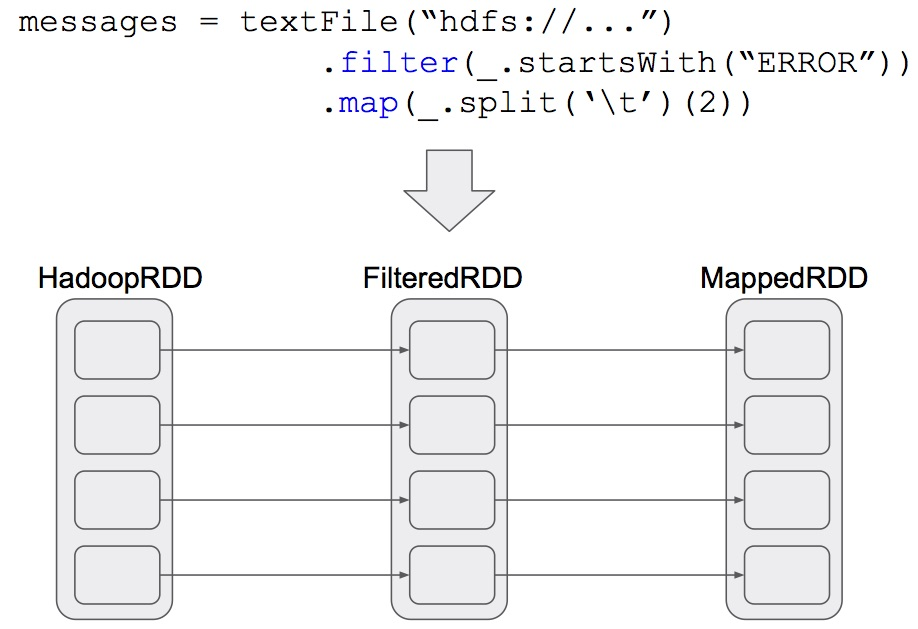
\includegraphics[width=0.7\linewidth]{figures/fault-tolerance.jpg}
\caption{RDDs track their lineage (graph of transformations that built them) to
rebuild lost data.}
\end{figure}
\end{frame}

\subsection{RDD vs DSM}
\begin{frame}
\begin{figure}
\centering
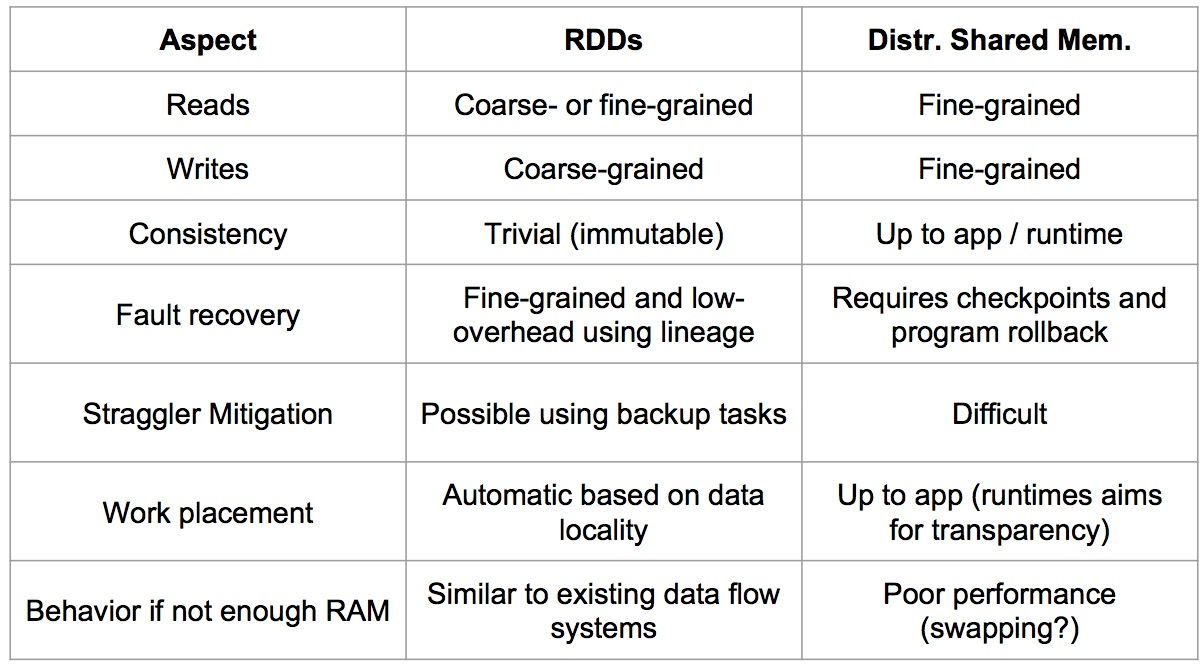
\includegraphics[width=0.9\linewidth]{figures/rdd-vs-dsm.jpg}
\caption{Comparison of RDDs with distributed shared memory.}
\end{figure}
\end{frame}

\subsection{RDDs Limitations}
\begin{frame}
\begin{itemize}
  \item Works best for batch applications that apply same operation to all
  elements of a dataset,
  \item Not well-suited for applications that do asynchronous fine-grained
  updates to shared state, e.g., storage system for a web application.
\end{itemize}
\end{frame}

